\chapter{Generieren von Testdaten}
\label{chap:generieren}

Das Generieren von Test-Daten ist kein neues Thema. Es gibt verschiedene Ans�tze daf�r. Einige Programme genieren
Massendaten. Die Erwartung ist, dass durch die Vielzahl zuf�lliger Daten auch alle Arten von Beziehungen ausreichend
generiert werden. Ein solcher Massendaten-Generator l�sst sich vergleichsweise leicht realisieren. 
F�r Unit-Tests mit �berschaubaren Test-Daten ist dieser Ansatz eher nicht geeignet.

Ein anderer Ansatz ist f�r Unit-Tests entgegenkommender. Dort werden Test-Daten anhand von konkreten Abfragen 
generiert. Allerdings ist es nicht Ziel der Arbeit, f�r jeden Test individuelle Daten zu generieren. Au�erdem k�nnen
Anfragen vom SUT auch abstrahiert werden, beispielsweise wenn ein Spring-Service verwendet wird.

F�r die Generierung von Test-Daten aus einem Datenbank-Modell bietet sich die erste Variante an. Da die Menge
der generierten Test-Daten gering gehalten werden soll, soll ein Algorithmus entwickelt werden, der Beziehungen
nicht rein zuf�llig modelliert. Stattdessen soll versucht werden, m�glichst alle Grenzf�lle zu ber�cksichtigen.
�quivalenzklassenbildung und Grenzwertanalyse sind ein bew�hrtes Vorgehen, um die Menge von Test-Daten zu
reduzieren.

Im Folgenden wird beschrieben, welche F�lle f�r verschiedene bin�re Beziehungen auf jeden Fall generiert werden
m�ssen.

\section{Generieren von Beziehungen}


	\subsection{1:1}
	
		\subsubsection{1..1:1..1}
		
		\begin{figure}[htbp]
			\centering
			 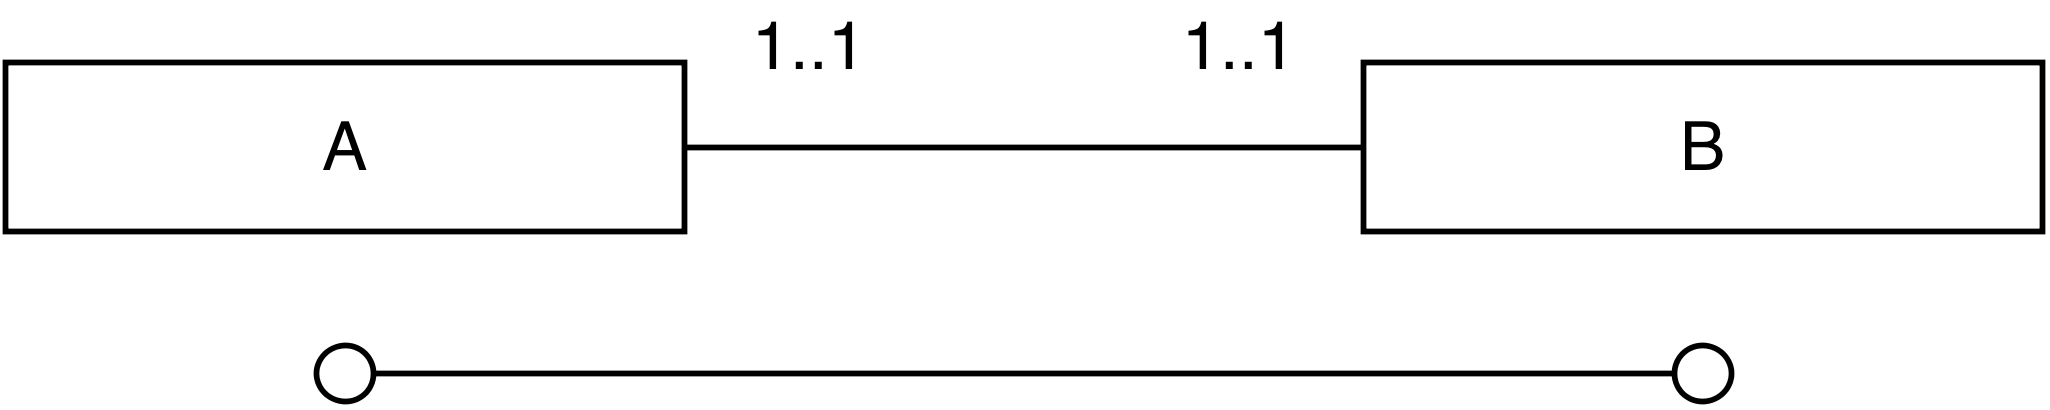
\includegraphics[width=0.55\textwidth]{images/generierung/1-1-to-1-1.png}
			\caption{Beziehungen nach dem Schema 1..1:1..1}\label{img:generierung:11to11}
		\end{figure}

		
		\subsubsection{0..1:1..1}

		\begin{figure}[htbp]
			\centering
			 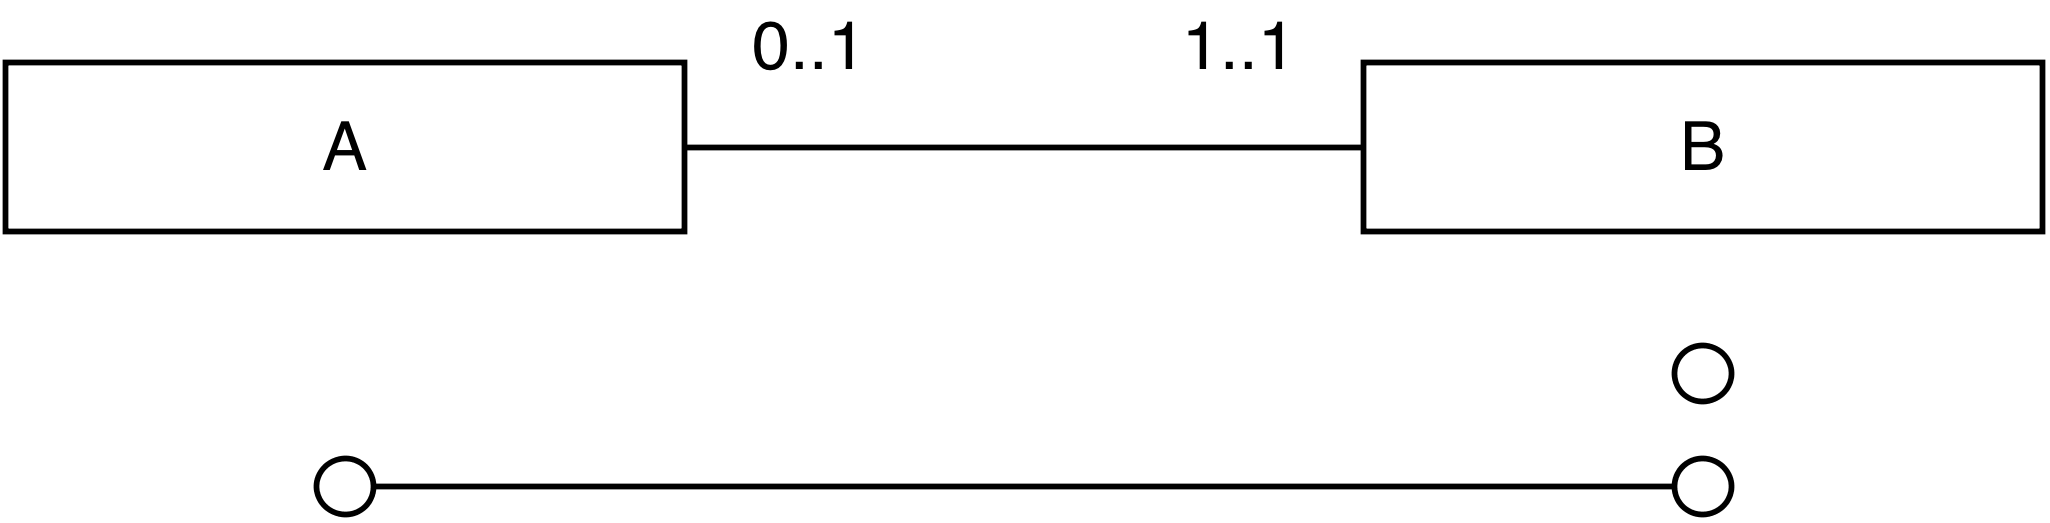
\includegraphics[width=0.55\textwidth]{images/generierung/0-1-to-1-1.png}
			\caption{Beziehungen nach dem Schema 0..1:1..1}\label{img:generierung:01to11}
		\end{figure}

		\subsubsection{0..1:0..1}

		\begin{figure}[htbp]
			\centering
			 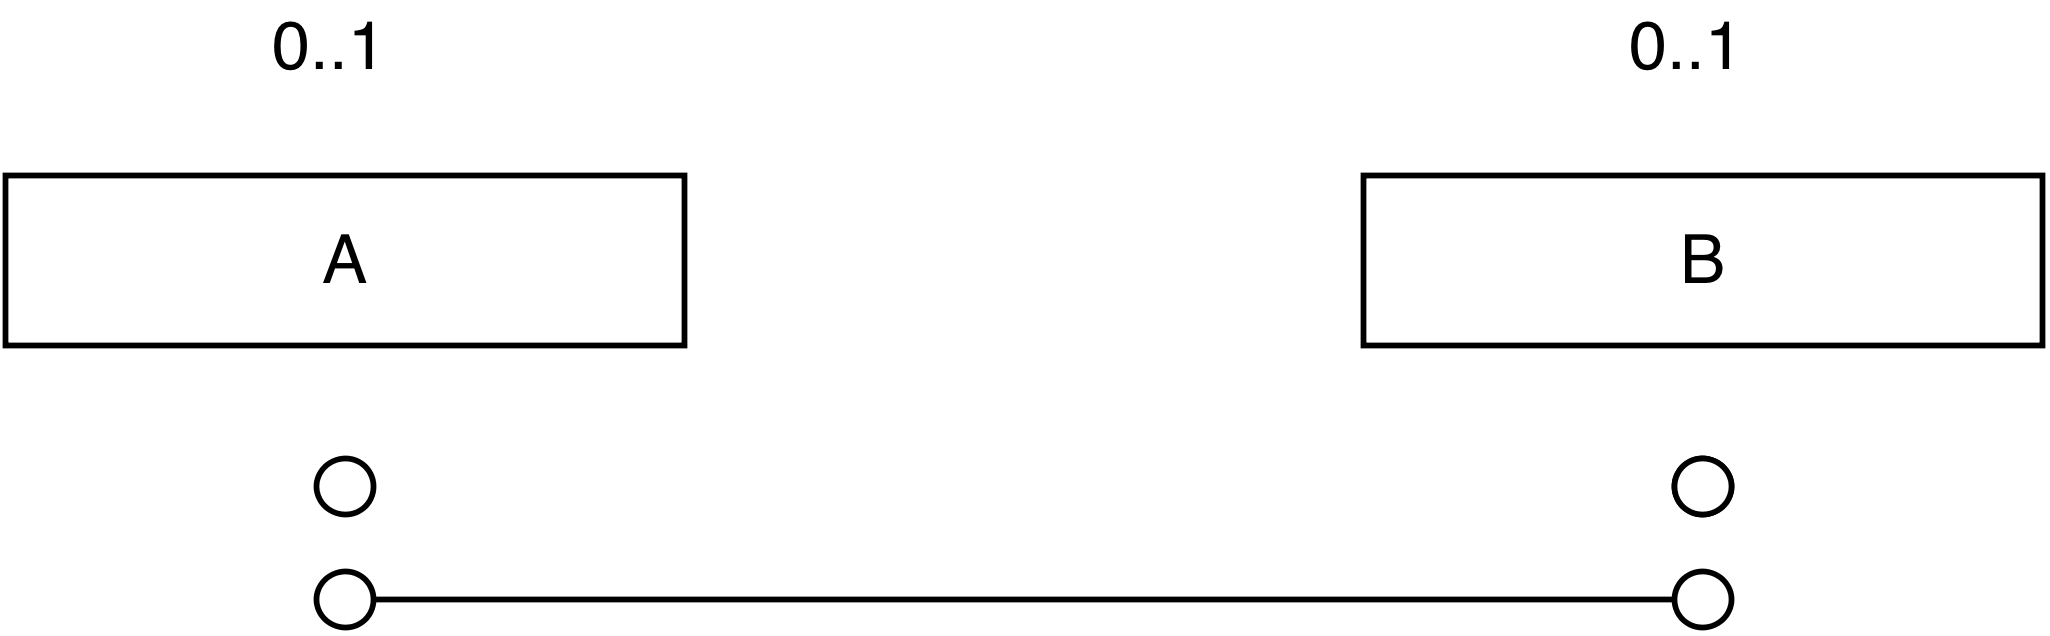
\includegraphics[width=0.55\textwidth]{images/generierung/0-1-to-0-1.png}
			\caption{Beziehungen nach dem Schema 0..1:0..1}\label{img:generierung:01to01}
		\end{figure}

	\subsection{1:n}

		\subsubsection{1..1:1..n}

		\begin{figure}[htbp]
			\centering
			 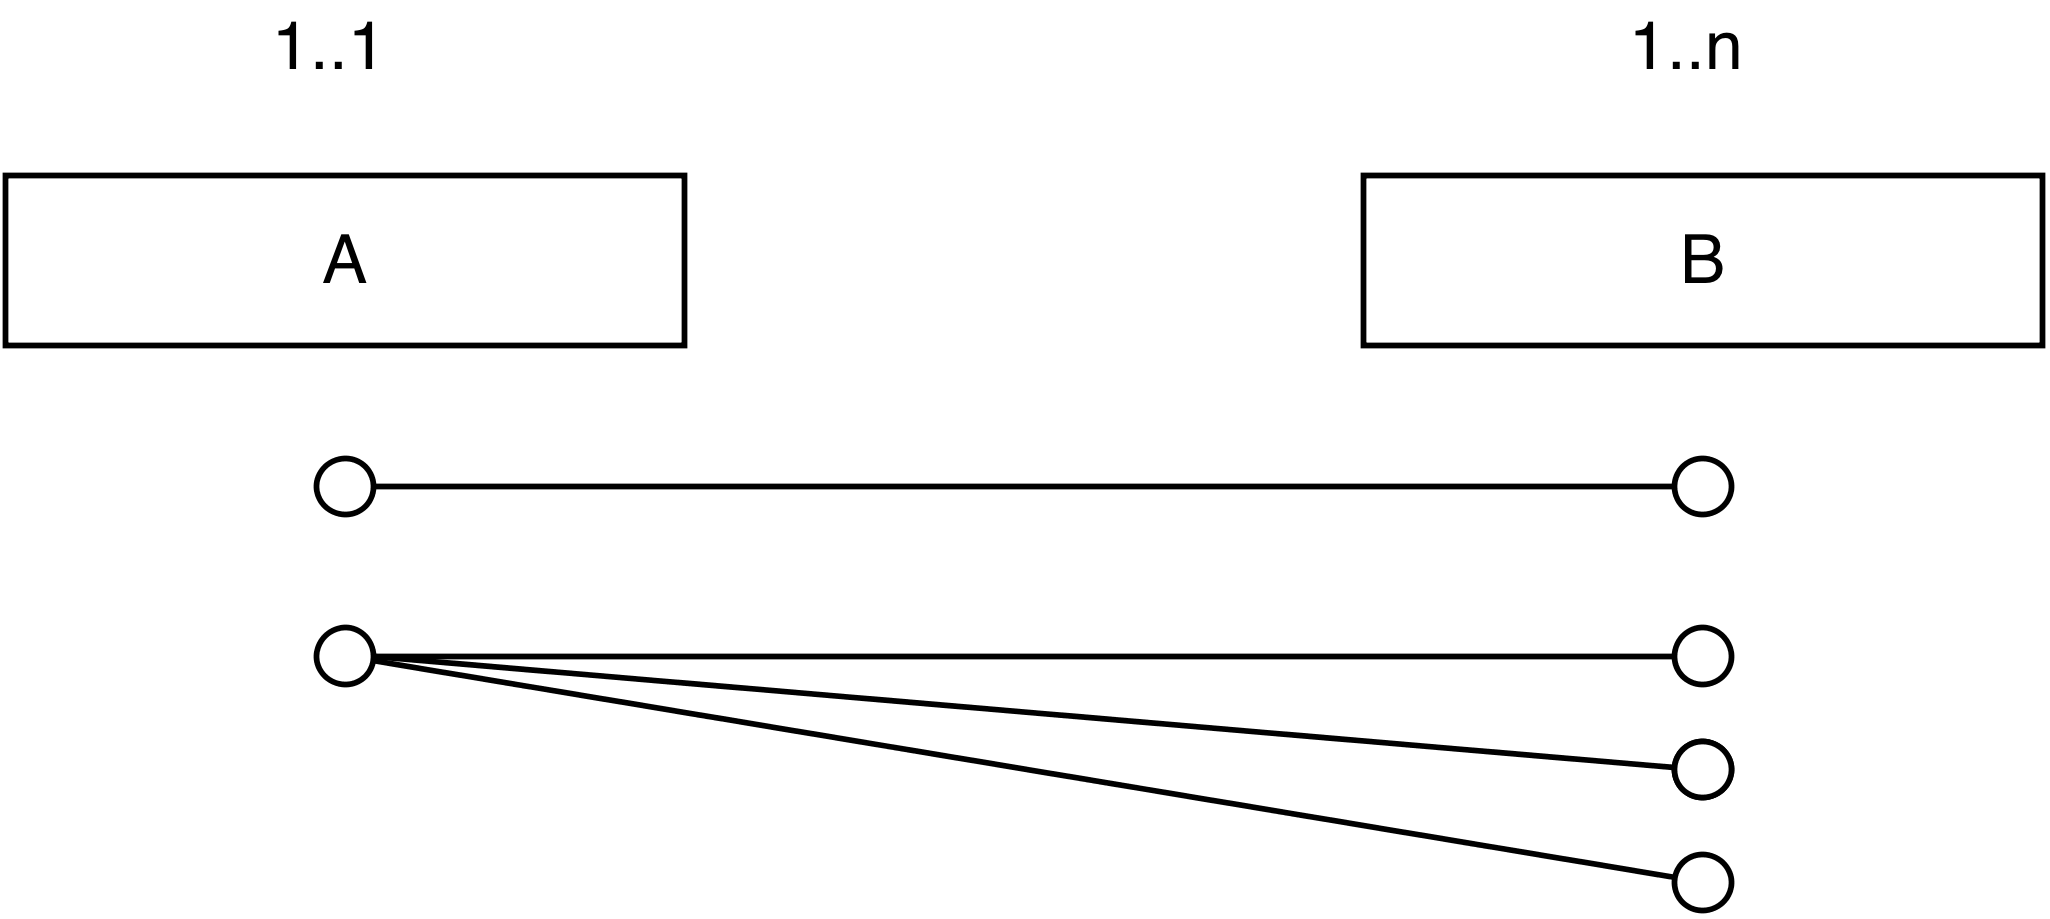
\includegraphics[width=0.55\textwidth]{images/generierung/1-1-to-1-n.png}
			\caption{Beziehungen nach dem Schema 1..1:1..n}\label{img:generierung:11to1n}
		\end{figure}

		\subsubsection{0..1:1..n}

		\begin{figure}[htbp]
			\centering
			 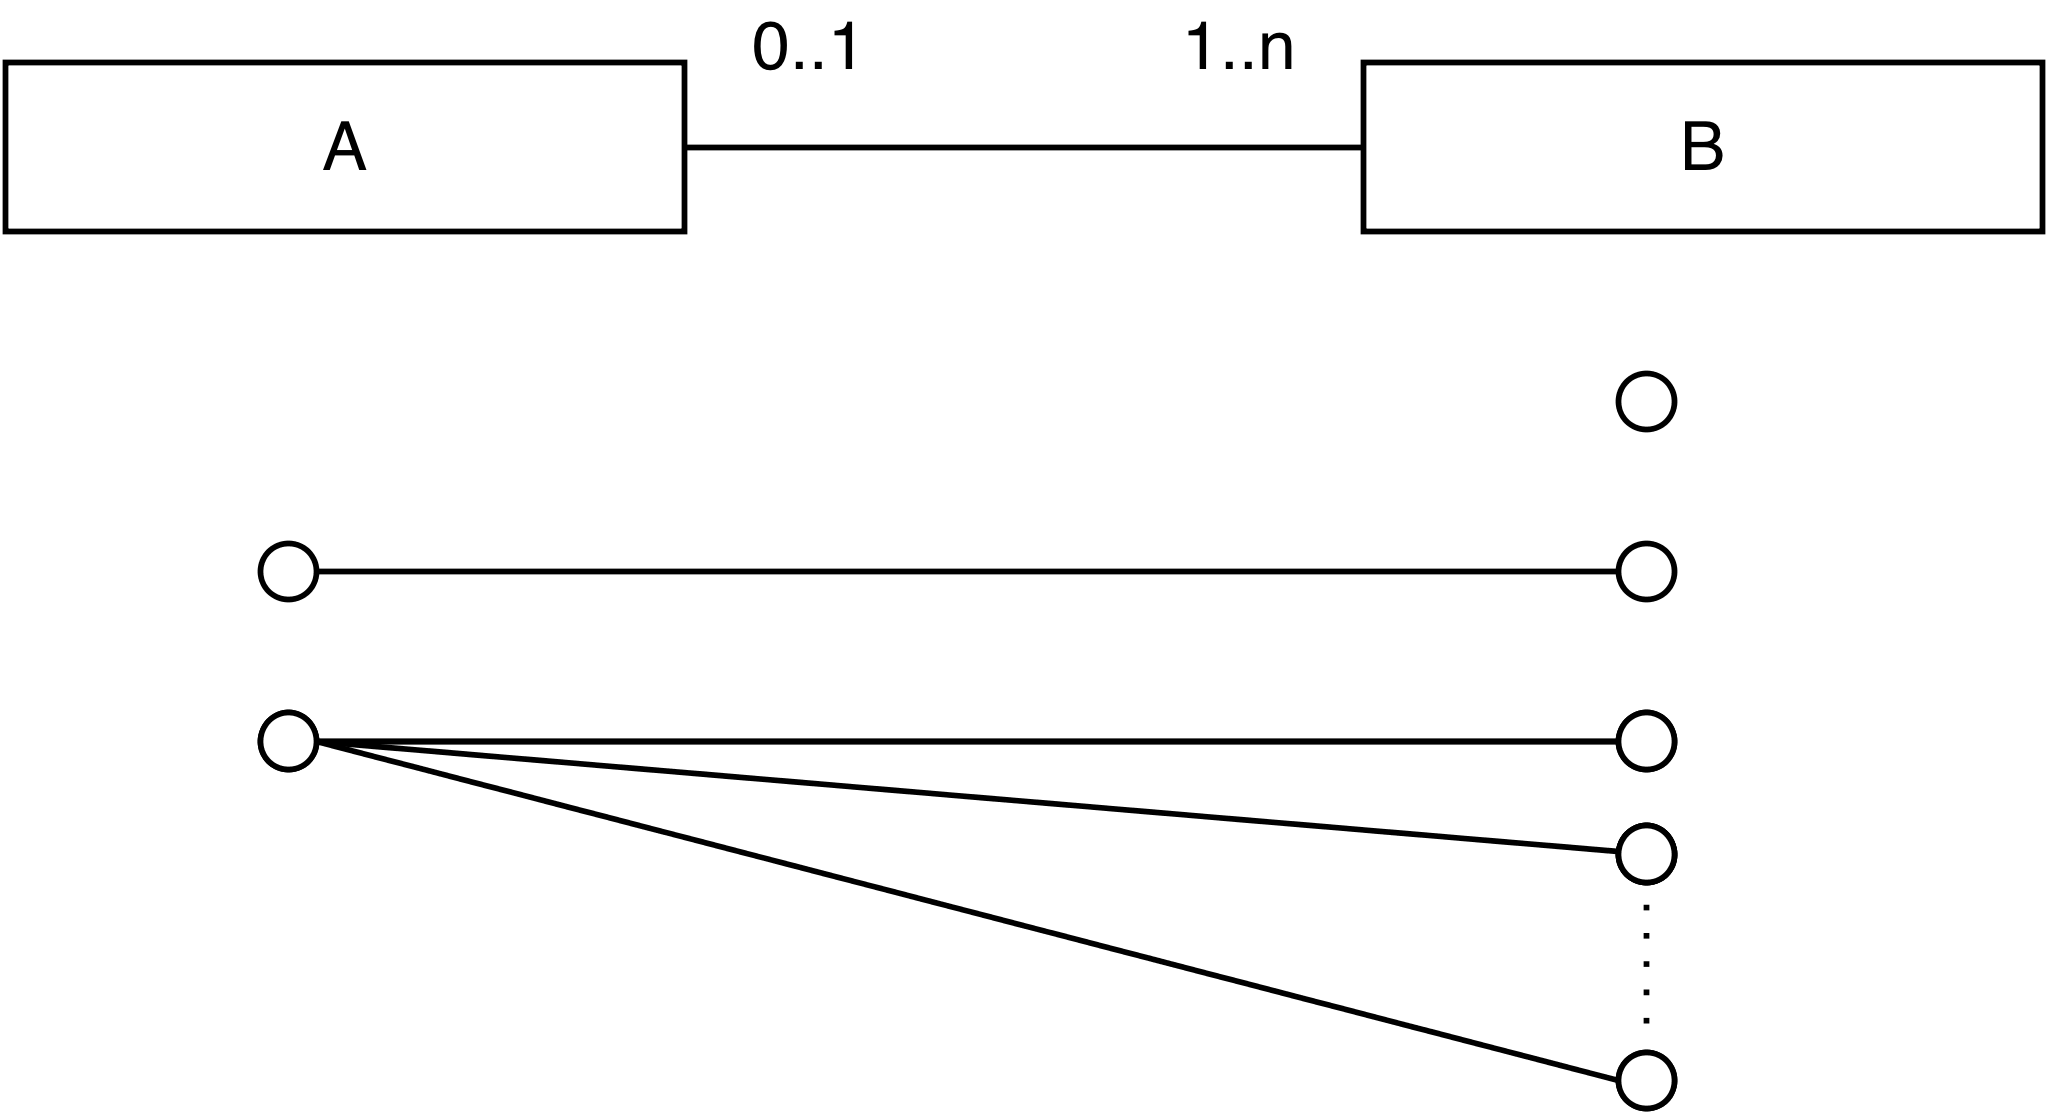
\includegraphics[width=0.55\textwidth]{images/generierung/0-1-to-1-n.png}
			\caption{Beziehungen nach dem Schema 0..1:1..n}\label{img:generierung:01to1n}
		\end{figure}
		
		\subsubsection{1..1:0..n}

		\begin{figure}[htbp]
			\centering
			 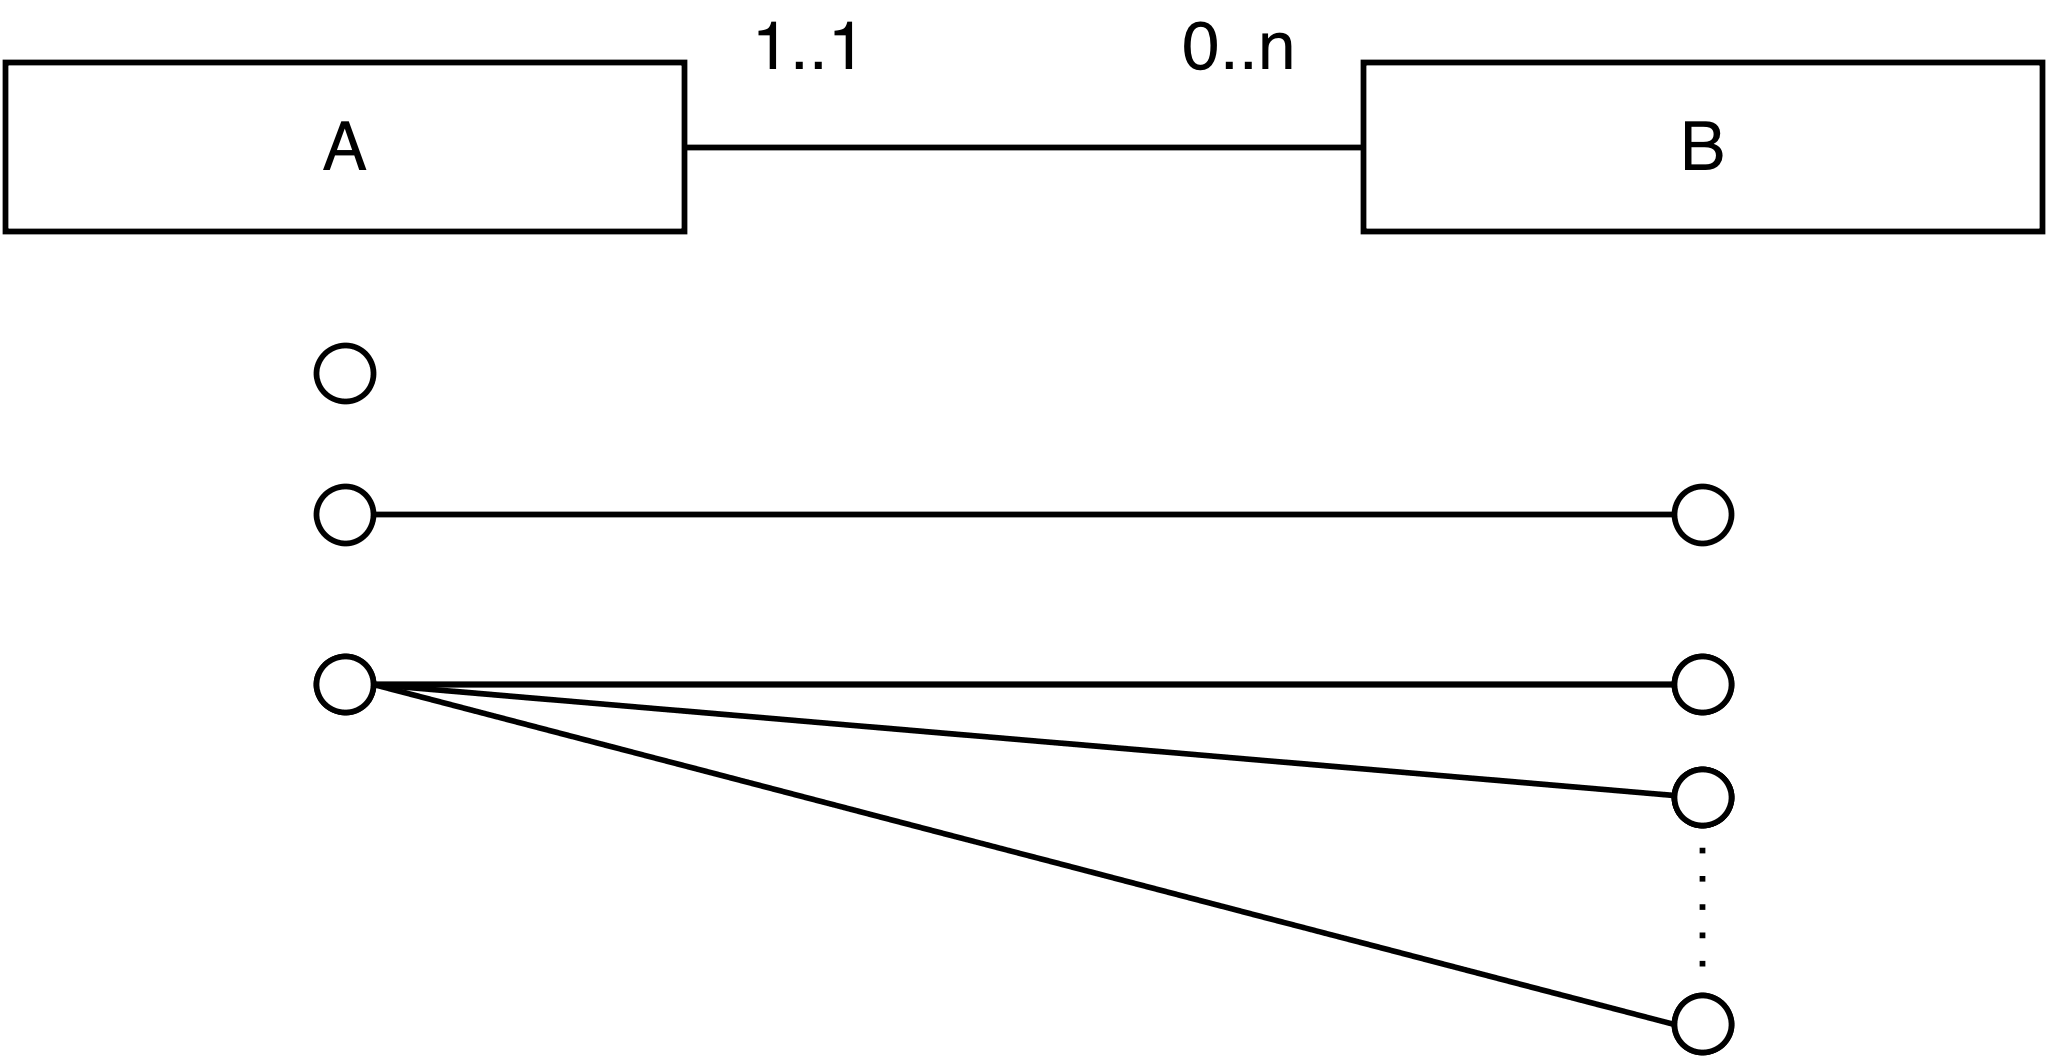
\includegraphics[width=0.55\textwidth]{images/generierung/1-1-to-0-n.png}
			\caption{Beziehungen nach dem Schema 1..1:0..n}\label{img:generierung:11to0n}
		\end{figure}

		\subsubsection{0..1:0..n}

		\begin{figure}[htbp]
			\centering
			 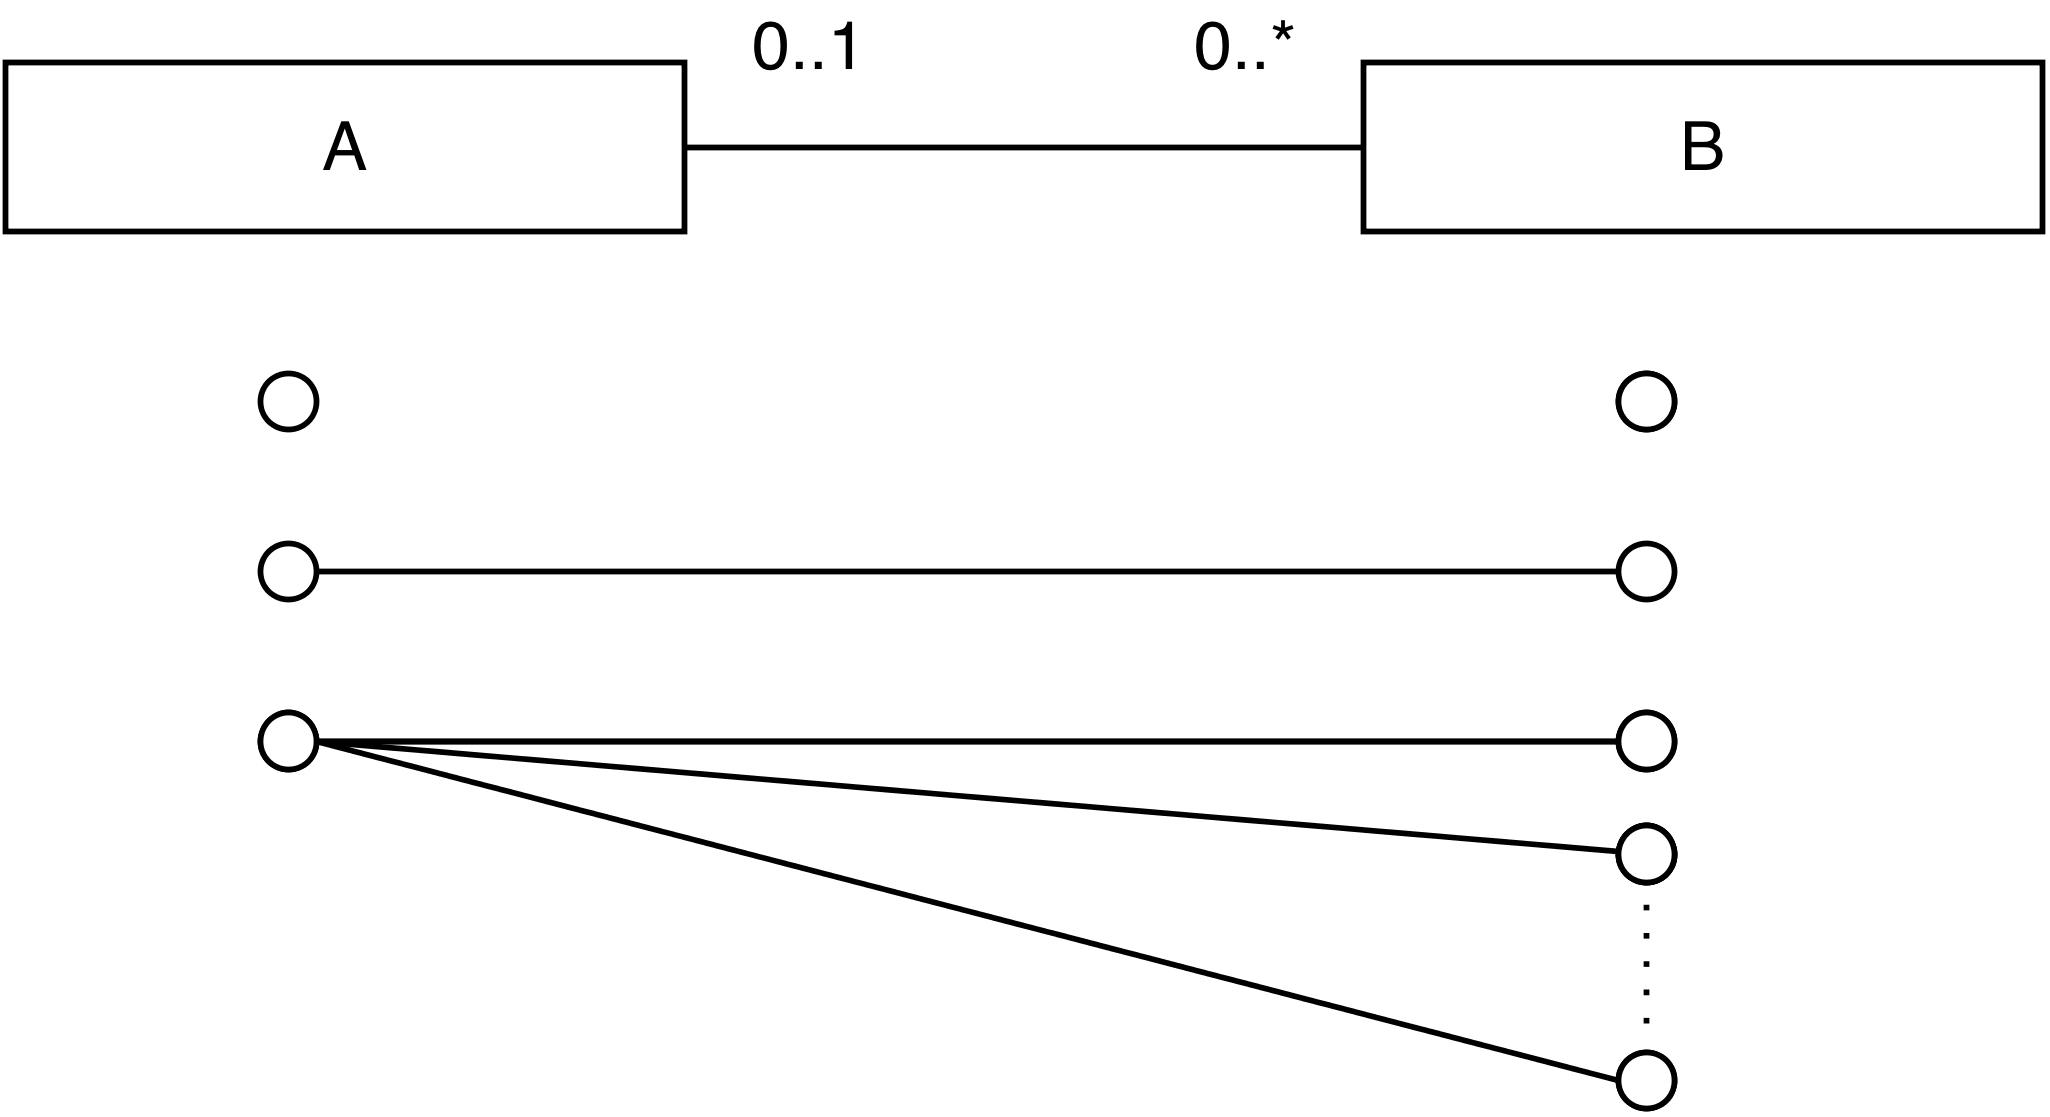
\includegraphics[width=0.55\textwidth]{images/generierung/0-1-to-0-n.png}
			\caption{Beziehungen nach dem Schema 0..1:0..n}\label{img:generierung:01to0n}
		\end{figure}

	\subsection{n:m}






Red Gate SQL Data Generator:
- Fragt Datenbank-Schema aus SQL-Server ab
- Modelliert Beziehungen(!), allerdings zuf�llig und bedeutungslos
- Anzahl generierter Zeilen pro Tabelle steuerbar
- Zufall pro Spalte �ber Seed steuerbar
- Eher f�r gro�e Datenmengen gedacht


DTM Data Generator
- Weniger bequem als Red Gate, z.B. keine Erkennung der Spaltentypen
- 



- Beziehungstypen, wie werden sie generiert
- Assoziative Tabellen

\section{Warum Generierung}
M�glichkeiten:
- Generierung
- Real-Daten, Extraktion, Anonymisierung (bei Unit-Tests wenig praktikabel, da Tests vor Inbetriebnahme laufen sollen)

Je nach Anwendungsfall unterschiedliche Data-Sets sinnvoll
- Unit-Tests eher klein
- Performance-Tests, Regressionstests eher gro�


\section{Erweiterungen am Modell}

\section{Der Algorithmus}
1. Start-Tabelle festlegen
2. wenn Tabelle noch nicht behandelt, dann
3. Kanten bestimmen und behandeln (ausgehende bevorzugt)
4. Schritte 2-4 rekursiv f�r die verbundene Tabelle wiederholen
5. Pr�fen ob alle Entit�ten g�ltige Beziehungen haben, ggf. Entit�ten erstellen

Assoziative Tabellen werden separat behandelt
Jede Kante und jede Tabelle wird nur ein mal in den Schritten 2-4 besucht


\section{Probleme}